\chapter{二元固液相图}\label{ch:b2:solid-liquid-diagrams}

锡在 \qty{232}{\degreeCelsius} 熔化，铅在 \qty{327}{\degreeCelsius} 熔化，
然而电工用的旧焊锡是两者的混合物，它的熔化温度为
\qty{182}{\degreeCelsius}，比两者都低。撒在路面上的盐能使冰熔化，
但只能降到约 \qty{-21}{\degreeCelsius}；在更冷的夜晚则毫无作用。
另一方面，铜和镍即使在固态时也能以任意比例互溶，
其合金的熔化温度范围位于两种金属熔点之间。
本章的相图说明：对每一对金属，冷却的液体中会结晶出哪些固体，
在什么温度下结晶，以及各固体的
含量——这正是每一次铸造、每一处焊接以及每一种
低熔点合金背后的知识。

\begin{recall}
\Cref{ch:b2:chemical-potential}：理想混合物中组分的化学势，
凝固点降低。\Cref{ch:b2:equilibrium-shifts}：自由度。
\Cref{ch:b2:liquid-vapour-diagrams}：二元相图、系线与杠杆
规则。本科一年级分册：金属键，置换型与间隙型
合金，晶体类型。
\end{recall}

\begin{omfigure}
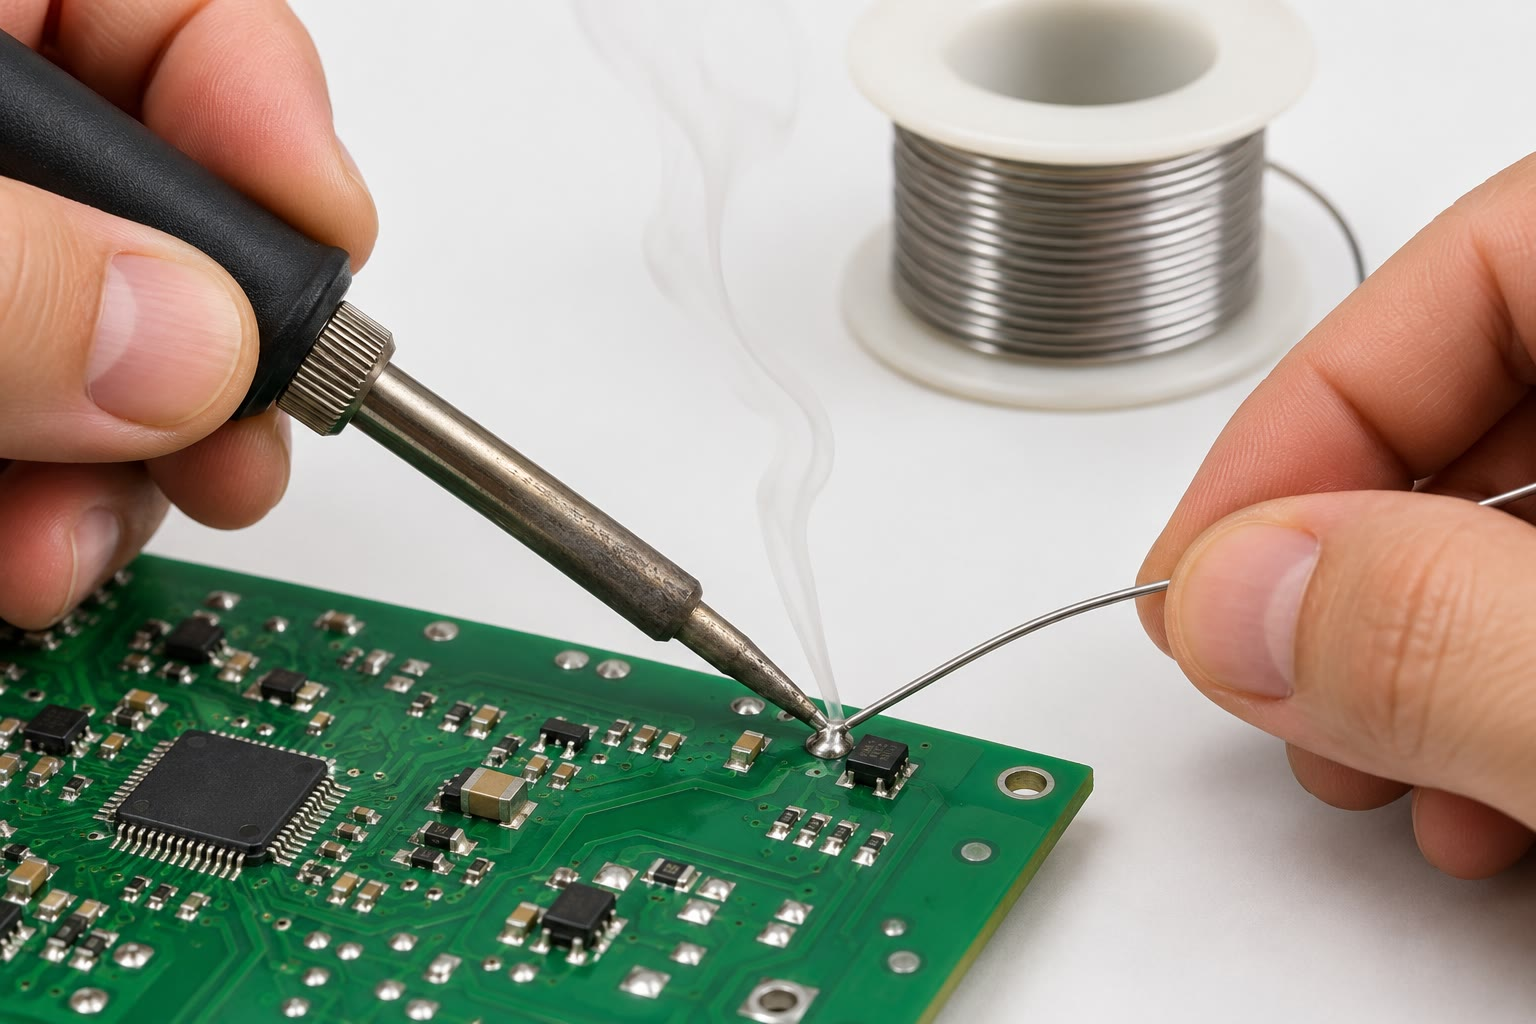
\includegraphics[width=0.6\linewidth]{images/book3/ai/b2-08-soldering.jpg}

{\small 电路板上焊接元件时，焊锡丝接触热的烙铁即熔化，
焊点在烙铁移开后一秒之内凝固
——因为该合金只在单一的较低温度下熔化。}
\end{omfigure}

\section{热分析}

\begin{definition}[热分析]\label{def:b2:solid-liquid-diagrams:cooling-curve}
\emph{热分析}\index{热分析}由样品在匀速加热或冷却过程中记录的温度，
确定其发生相变的温度。
温度随时间变化的记录，
在缓慢冷却时称为\emph{冷却曲线}\index{冷却曲线}。
\end{definition}

在远离任何相变的区域，样品平稳地冷却。当固体开始
结晶时，结晶放出的热量会减缓冷却：曲线出现一个
斜率出现转折，或在某一恒定温度下停留一段时间——即
\textit{平台}——若凝固在固定温度下发生。

\begin{proposition}[平台]\label{prop:b2:solid-liquid-diagrams:plateaus}
在压强一定时，纯净物在恒定温度下凝固，
二元液体中若有两种固体同时结晶，亦然。
只析出一种固体的二元液体则在一个温度范围内凝固。
\end{proposition}

\begin{proof}
压强固定，自由度为 $v = n - r + 1 - \varphi$。纯净
物，液相加固相：$v = 1 + 1 - 2 = 0$。二元体系，液相加两种固相：
$v = 2 + 1 - 3 = 0$。二元体系，液相加一种固相：$v = 2 + 1 - 2 = 1$，
温度随液相组成变化。自由度为 0 意味着
只要各相同时存在，温度便不能改变：所移走的热量
由凝固过程补足，直至某一相消失。
\end{proof}

\begin{omfigure}
\begin{tikzpicture}[font=\small, x=0.55cm, y=0.05cm]
  \foreach \dx/\name in {0/纯金属, 9/{混合物：先析出一种固体}, 18/低共熔混合物} {
    \draw[->] (\dx,0) -- (\dx+7.5,0) node[below left, font=\scriptsize] {$t$};
    \draw[->] (\dx,0) -- (\dx,62) node[above, font=\scriptsize] {$T$};
    \node[font=\scriptsize] at (\dx+3.8,-8) {\name};
  }
  % pure: cool, plateau at 40, cool
  \draw[omDef, thick] (0,58) .. controls (1,48) and (1.6,42) .. (2,40) -- (4.5,40) .. controls (5.2,32) and (6,24) .. (7,20);
  \node[font=\scriptsize, anchor=south] at (3.25,40.5) {平台};
  % mixture: cool, break at 48, slow fall, plateau at 30, cool
  \draw[omDef, thick] (9,58) .. controls (9.6,53) and (9.9,50) .. (10.2,48)
     .. controls (11,42) and (11.6,35) .. (12.3,30) -- (14.2,30) .. controls (14.9,23) and (15.6,17) .. (16.5,14);
  \node[font=\scriptsize, anchor=west] at (10.4,49.5) {转折};
  \node[font=\scriptsize, anchor=south] at (13.25,30.5) {低共熔点};
  % eutectic: plateau at 30
  \draw[omDef, thick] (18,58) .. controls (19,46) and (19.8,36) .. (20.5,30) -- (24,30) .. controls (24.7,23) and (25.4,17) .. (26.2,14);
  \node[font=\scriptsize, anchor=south] at (22.25,30.5) {平台};
\end{tikzpicture}

{\small 冷却曲线示意图。纯金属在平台上凝固。混合物
在第一个固体析出时斜率出现转折，随后缓慢降温，
液体在一定温度范围内凝固，随后是低共熔平台。
低共熔组成的液体在
单一平台上凝固，与纯净物一样。}
\end{omfigure}

\begin{method}[由冷却曲线绘制相图]\label{met:b2:solid-liquid-diagrams:diagram-from-curves}
\begin{enumerate}
  \item 记录一系列组成的冷却曲线，
        包括纯组分在内。
  \item 在（组成，温度）图上，对每一组成描出
        首次转折（开始结晶）的温度以及
        各平台的温度。
  \item 连接开始结晶的点，得液相线。连接
        凝固终点，得固相线。在许多组成下于同一温度出现的平台
        温度，即为一条不变线（低共熔线）。
  \item 低共熔平台的长度在低共熔组成处最大，
        由此可确定该组成。
\end{enumerate}
\end{method}

\section{固态中的完全互溶}

\begin{definition}[固溶体]\label{def:b2:solid-liquid-diagrams:solid-solution}
\emph{固溶体}\index{固溶体}是一种组成可变的单一晶相，
其中一种组分的原子取代另一种组分的原子，占据同一晶格的格点（置换型），
或占据该晶格的
空穴（间隙型）。
\end{definition}

铜和镍具有相同的面心立方结构，原子半径相近，
因此在任意组成下都形成置换型固溶体。

\begin{definition}[液相线与固相线]\label{def:b2:solid-liquid-diagrams:liquidus}
在固液相图中，\emph{液相线}\index{液相线}是这样一条曲线，
其上方全为液相，它给出与固体平衡的液相的
组成。\emph{固相线}\index{固相线}是这样一条曲线，
其下方全为固相；若固相为溶液，它给出与液相平衡的固相的
组成。
\end{definition}

\begin{proposition}[透镜]\label{prop:b2:solid-liquid-diagrams:lens}
若两组分在液相与固相中均形成理想溶液，
则液相线与固相线连接两个熔点，并围成一个
透镜形两相区；在每一温度下，各组分的摩尔分数 $x_i$
在液相与固相中满足如下关系：
\[
  \frac{x_i^{\ell}}{x_i^{s}} = \exp\left[-\frac{\Delta_{\text{fus}}H_i}{R}\left(\frac1T - \frac1{T_i^*}\right)\right] .
\]
\end{proposition}

\begin{proof}
组分 $i$ 在两相中的化学势相同，$\mu_i^{*,s} +
RT\ln x_i^s = \mu_i^{*,\ell} + RT\ln x_i^\ell$，于是 $RT\ln(x_i^\ell/x_i^s) =
-(\mu_i^{*,\ell} - \mu_i^{*,s}) = -\Delta_{\text{fus}}G_i(T)$，
若 $\Delta_{\text{fus}}H_i$ 为常数，则 $\Delta_{\text{fus}}G_i = \Delta_{\text{fus}}H_i(1 - T/T_i^*)$。
结合各相中的 $x_1 + x_2 = 1$，这两个关系式确定了
每一 $T$ 下的两组成（图中由数值求解）；
所得曲线呈透镜形，此点在本阶段不加证明地承认。
\end{proof}

\begin{omfigure}
\begin{tikzpicture}
\begin{axis}[omphase, width=0.62\linewidth, height=7cm, ymin=1050, ymax=1480,
  xlabel={$x$（镍）}, ylabel={$T$（\unit{\degreeCelsius}）}]
\addplot[omliquidus] table[x=xl, y=T] {figdata/out/bachelor-2-solid-liquid-a.dat};
\addplot[omsolidus] table[x=xs, y=T] {figdata/out/bachelor-2-solid-liquid-a.dat};
\draw[tieline] (axis cs:0.541,1300) -- (axis cs:0.609,1300);
\fill (axis cs:0.58,1300) circle (1.3pt);
\node[font=\scriptsize] at (axis cs:0.25,1400) {液相};
\node[font=\scriptsize] at (axis cs:0.8,1150) {固溶体};
\node[font=\scriptsize, anchor=east] at (axis cs:0.5,1330) {液相线};
\node[font=\scriptsize, anchor=west] at (axis cs:0.66,1290) {固相线};
\node[font=\scriptsize, anchor=west] at (axis cs:0.03,1080) {\qty{1085}{\degreeCelsius}};
\draw[black!50] (axis cs:0.005,1084) -- (axis cs:0.03,1080);
\node[font=\scriptsize, anchor=south east] at (axis cs:1.0,1456) {\qty{1455}{\degreeCelsius}};
\end{axis}
\end{tikzpicture}

{\small 铜–镍，按固相与液相均为理想溶液计算，依据
两金属的熔点与熔化焓。在
\qty{1300}{\degreeCelsius} 时，组成为 0.58 的合金分为组成 0.541 的液相
和组成 0.609 的固相（虚线为连接线）。}
% ledger: tfus:Cu, dfus:Cu, tfus:Ni, dfus:Ni
\end{omfigure}

\begin{method}[读固液相图]\label{met:b2:solid-liquid-diagrams:read-solid-liquid}
\begin{enumerate}
  \item 沿总组成的竖直线，自液相区向下
        行进。
  \item 在液相线上出现第一个固体，其组成在
        连接线的另一端读取（即固相线或某一纯组分）。
  \item 在两相区，读取连接线两端的两个组成，
        并用杠杆规则求两相比例：按物质的量计时用摩尔分数，
        按质量计时用质量分数。
  \item 在水平不变线上，温度保持不变，直至一相
        消失；其下方则读取新的一对相。
\end{enumerate}
\end{method}

\begin{example}[\qty{1300}{\degreeCelsius} 时的合金]\label{ex:b2:solid-liquid-diagrams:lever}
对镍的摩尔分数为 0.58 的合金，在 \qty{1300}{\degreeCelsius} 下，
固相中原子所占的比例为 $(0.58 - 0.541)/(0.609 - 0.541) = 0.57$。
最先出现的固体（在 \qty{1315}{\degreeCelsius} 附近）镍含量高于合金，
而最后的液体则较低。
\end{example}

相图描述的是平衡状态，而固体中达到平衡很慢：最先析出的晶体
富镍，随着液体的变化，被镍含量越来越低的
外层所覆盖，固相中的扩散来不及使其均匀化。冷却迅速的铸件
则由\textit{芯部偏析的}晶体组成，其组成从中心到
边缘逐渐变化；在固相线以下长时间加热可使其均匀化。

\section{固相中不互溶：低共熔点}

当两种固体完全不互溶时，每一组分均以纯态结晶，
液相线则有两支，各对应一种固体。

\begin{theorem}[施罗德–范拉尔]\label{thm:b2:solid-liquid-diagrams:schroder}
若组分 A 自理想液态混合物中以纯态结晶，
则出现固体 A 的液相线由下式给出
\[
  \ln x_A = -\frac{\Delta_{\text{fus}}H_A}{R}\Big(\frac1T - \frac1{T_A^*}\Big),
\]
其中 $x_A$ 为液相中 A 的摩尔分数，$T_A^*$ 与
$\Delta_{\text{fus}}H_A$ 分别为纯 A 的熔点与熔化焓
（视为常数）。
\end{theorem}

\begin{proof}
平衡时，纯固体 A 的化学势等于液相中 A 的化学势：
$\mu_A^{*,s}(T) = \mu_A^{*,\ell}(T) + RT\ln x_A$。由此 $R\ln x_A =
-\Delta_{\text{fus}}G_A(T)/T$。由吉布斯--亥姆霍兹关系，$d(\Delta_{\text{fus}}G_A/T)/
dT = -\Delta_{\text{fus}}H_A/T^2$；自 $T_A^*$
处（此时 $\Delta_{\text{fus}}G_A = 0$）积分至 $T$，得 $\Delta_{\text{fus}}G_A/T =
\Delta_{\text{fus}}H_A(1/T - 1/T_A^*)$.
\end{proof}

对稀溶液，$\ln x_A = \ln(1 - x_B) \approx -x_B$，且 $1/T -
1/T_A^* \approx -\Delta T/T_A^{*2}$，得 $\Delta T = RT_A^{*2}x_B/\Delta_{\text{fus}}H_A$，
即 \cref{ch:b2:chemical-potential}中的凝固点降低定律。对苯（$T^* =
\qty{278.64}{K}$, $\Delta_{\text{fus}}H = \qty{9.87}{kJ/mol}$, $M =
\qty{78.11}{g/mol}$），凝固点降低常数 $RT^{*2}M/\Delta_{\text{fus}}H$
算得为 \qty{5.11}{K.kg/mol}。
% ledger: tfus:benzene, dfus:benzene

\begin{definition}[低共熔点]\label{def:b2:solid-liquid-diagrams:eutectic}
二元系统的\emph{低共熔点}\index{低共熔点}是
液体同时与两种固体处于平衡的点；它是
相图中该部分液体能存在的最低温度。
低共熔组成的液体，以及它凝固所成的两种固体的细密混合物，
统称为
\emph{低共熔混合物}\index{低共熔混合物}。
\end{definition}

\begin{corollary}[低共熔点即两支液相线的交点]\label{cor:b2:solid-liquid-diagrams:eutectic}
对固相中不互溶、液相为理想溶液的两个组分，
低共熔温度 $T_E$ 及组成为
$x_A(T_E) + x_B(T_E) = 1$ 的解，每个 $x$ 由其对应固相的
施罗德–范拉尔方程给出。
\end{corollary}

\begin{proof}
在低共熔点处，液相同时被两种固体饱和：
它同时位于两条分支上，从 A 与从 B 读出的组成相同。
\end{proof}

\begin{omfigure}
\begin{tikzpicture}
\begin{axis}[omphase, width=0.62\linewidth, height=6.5cm, ymin=-25, ymax=85,
  xlabel={$x$（萘）}, ylabel={$T$（\unit{\degreeCelsius}）}]
\addplot[omliquidus] table[x=x, y=T] {figdata/out/bachelor-2-solid-liquid-b-benzene.dat};
\addplot[omliquidus] table[x=x, y=T] {figdata/out/bachelor-2-solid-liquid-b-naphthalene.dat};
\draw[thick] (axis cs:0,-3.55) -- (axis cs:1,-3.55);
\fill (axis cs:0.133,-3.55) circle (1.5pt);
\node[font=\scriptsize, anchor=north] at (axis cs:0.133,-4.5) {E};
\node[font=\scriptsize] at (axis cs:0.45,72) {液体};
\node[font=\scriptsize, align=center] at (axis cs:0.65,22) {液体 + 固态 \\ 萘};
\node[font=\scriptsize, anchor=south west] at (axis cs:0.08,45) {液体 + 固态苯};
\draw[thin] (axis cs:0.12,45) -- (axis cs:0.06,0.8);
\node[font=\scriptsize] at (axis cs:0.55,-15) {固态苯 + 固态萘};
\end{axis}
\end{tikzpicture}

{\small 苯–萘，由各固相的施罗德–范拉尔
方程计算。两支曲线在低共熔点 E 处相交，
\qty{-3.5}{\degreeCelsius}、萘组成 0.13，其下全部为固体。}
% ledger: tfus:benzene, dfus:benzene, tfus:naphthalene, dfus:naphthalene
\end{omfigure}

\begin{example}[苯–萘混合物的冷却]\label{ex:b2:solid-liquid-diagrams:naphthalene}
萘的摩尔分数为 0.5 的液体冷却，直至
液相线萘分支上约 \qty{46}{\degreeCelsius} 处，纯固态萘
开始结晶。液体失去萘，沿分支下降；
在 \qty{-3.5}{\degreeCelsius} 处到达低共熔点，其余部分
于恒温下凝固为低共熔混合物。由杠杆规则，
刚高于低共熔点时，固态萘的物质的量分数为 $(0.5 - 0.133)/(1 - 0.133) =
42~\%$，低共熔液体为 58~\%。
\end{example}

\begin{proposition}[低共熔平台的长度]\label{prop:b2:solid-liquid-diagrams:plateau-length}
质量相同的样品以相同的散热速率冷却时，
低共熔平台的时长正比于到达低共熔点的液体量，
在低共熔组成时最大，对
纯组分则为零。
\end{proposition}

\begin{proof}
平台上温度恒定：移去的热量 $\Phi\,\Delta t$
（速率 $\Phi$ 恒定），等于低共熔液体凝固放出的热量
$m_E\,\Delta_{\text{fus}}h_E$。于是 $\Delta t = m_E\,\Delta_{\text{fus}}h_E/
\Phi$，即正比于低共熔液体的质量 $m_E$，
由杠杆规则给出。
\end{proof}

\section{部分互溶与确定化合物}

多数金属对在固态下既非完全互溶，
也非完全不互溶：每种金属都能溶入少量另一种。铅最多可溶入
19~\% 的锡（按质量计），锡最多溶入 3.4~\% 的铅。此时相图中有两个固溶体
(Pb) 与 (Sn)，以及二者之间的低共熔点；低共熔线不再
延伸到相图两侧，而止于固溶体的
极限处。

\begin{omfigure}
\begin{tikzpicture}[font=\small, x=0.075cm, y=0.022cm]
  \draw[->] (0,0) -- (106,0) node[right] {\% Sn（质量分数）};
  \draw[->] (0,0) -- (0,360) node[above] {$T$（\unit{\degreeCelsius}）};
  \foreach \t in {100,200,300} \draw (0,\t) -- (-1.5,\t) node[left, font=\scriptsize] {\t};
  \foreach \w in {0,20,40,60,80,100} \draw (\w,0) -- (\w,-5) node[below, font=\scriptsize] {\w};
  % invariant points (NIST): Pb 327.5, Sn 231.9, eutectic 182.2 at 62.13; limits 18.91 and 96.59
  \draw[omliquidus] (0,327.5) .. controls (25,290) and (45,235) .. (62.13,182.2);
  \draw[omliquidus] (100,231.9) .. controls (85,215) and (72,200) .. (62.13,182.2);
  \draw[omsolidus] (0,327.5) .. controls (8,280) and (14,220) .. (18.91,182.2);
  \draw[omsolidus] (100,231.9) .. controls (98.5,215) and (97.5,200) .. (96.59,182.2);
  \draw[thick] (18.91,182.2) -- (96.59,182.2);
  \draw[omsolidus, densely dashed] (18.91,182.2) .. controls (12,120) and (6,60) .. (3,20);
  \draw[omsolidus, densely dashed] (96.59,182.2) .. controls (98.5,120) and (99.3,60) .. (99.6,20);
  \fill (62.13,182.2) circle (1.5pt);
  \fill (18.91,182.2) circle (1.2pt); \fill (96.59,182.2) circle (1.2pt);
  \node[anchor=south, font=\scriptsize] at (62.13,186) {E};
  \node[font=\scriptsize] at (55,300) {液体};
  \node[font=\scriptsize] at (6,150) {(Pb)};
  \node[font=\scriptsize] at (103,140) {(Sn)};
  \node[font=\scriptsize] at (28,235) {L + (Pb)};
  \node[font=\scriptsize] at (84,192) {L + (Sn)};
  \node[font=\scriptsize] at (55,100) {(Pb) + (Sn)};
  % cooling path at 40 %
  \draw[->, omProp, thick] (40,340) -- (40,30);
  \node[font=\scriptsize, omProp, anchor=south] at (40,342) {40~\%};
  \node[font=\scriptsize, anchor=north east] at (16.6,179) {18.9};
  \node[font=\scriptsize, anchor=north] at (62.13,178) {62.1};
  \node[font=\scriptsize, anchor=north east] at (95.8,178) {96.6};
  \node[font=\scriptsize, anchor=west] at (101,182.2) {\qty{182.2}{\degreeCelsius}};
\end{tikzpicture}

{\small 铅–锡相图，画出了其不变点：熔点
分别为铅（\qty{327.5}{\degreeCelsius}）和锡（\qty{231.9}{\degreeCelsius}），
低共熔点 E 位于 \qty{182.2}{\degreeCelsius}，含锡 62.1~\%，固溶体
在低共熔温度下的极限（含锡 18.9~\% 和 96.6~\%）。曲线
位于这些点之间，以及低共熔温度以下的虚线溶解度极限，
均为示意画法。箭头表示含锡 40~\% 焊料的冷却。}
% ledger: eut:Pb-Sn.T, eut:Pb-Sn.wL, eut:Pb-Sn.wPb, eut:Pb-Sn.wSn, tfus:Pb, tfus:Sn
\end{omfigure}

含锡 40~\% 的焊料在液相线处开始凝固，析出
富铅固溶体（Pb）的晶体，液相中锡的含量不断升高，直至
\qty{182.2}{\degreeCelsius}时，液相达到低共熔组成，并凝固为
细密的（Pb）与（Sn）交替片层组成的混合物，包绕着初生晶体。

\begin{omfigure}
\begin{tikzpicture}[font=\small]
  \begin{scope}
    \clip (0,0) circle (2.2);
    \fill[gray!20] (-2.3,-2.3) rectangle (2.3,2.3);
    \foreach \k in {-24,...,24} \draw[gray!65, line width=1.1pt] (-2.4+0.2*\k,-2.4) -- ++(55:6);
    \foreach \cx/\cy/\r/\a in {-0.9/0.8/0.55/10, 0.7/1.0/0.45/40, 0.2/-0.6/0.6/-20, -1.1/-0.9/0.4/70, 1.3/-0.3/0.35/5} {
      \fill[omDef!35, draw=omDef, rotate around={\a:(\cx,\cy)}] (\cx,\cy) ellipse ({\r} and {0.7*\r});
    }
  \end{scope}
  \draw[thick] (0,0) circle (2.2);
  \draw[<-, omProp, thick] (0.7,1.0) -- (3.0,1.6) node[right, text=black] {初生（Pb）晶体};
  \draw[<-, omProp, thick] (1.6,0.9) -- (3.0,0.5) node[right, text=black, align=left] {低共熔混合物：交替的 \\ （Pb）与（Sn）片层};
\end{tikzpicture}

{\small 含锡 40~\% 焊料缓慢冷却后的显微组织示意：
（Pb）初生晶体形成于液相线与低共熔温度之间，
分布于低共熔混合物基体中，该基体由两种固溶体的细薄片
交替排列而成。}
\end{omfigure}

\begin{definition}[确定化合物]\label{def:b2:solid-liquid-diagrams:defined-compound}
称\emph{确定化合物}\index{确定化合物}为
由两种组分形成、组成固定为 $\mathrm{A}_a\mathrm{B}_b$ 的固体。它
表现为\emph{同成分熔融}\index{同成分熔融}，即熔化成与自身组成相同的液体，
此时液相线在该组成处取极大值。
\end{definition}

具有同成分熔融的化合物将相图一分为二：一半是 A 与
$\mathrm{A}_a\mathrm{B}_b$ 构成的，另一半是 $\mathrm{A}_a\mathrm{B}_b$ 与 B 构成的，二者
都是独立的相图，各有其低共熔点。以摩尔分数读取的极大值组成，
即给出该化合物的化学式。

\begin{omfigure}
\begin{tikzpicture}[font=\small, x=6cm, y=0.05cm]
  \draw[->] (0,0) -- (1.06,0) node[right] {$x_{\mathrm B}$};
  \draw[->] (0,0) -- (0,95) node[above] {$T$};
  \node[below, font=\scriptsize] at (0,0) {A}; \node[below, font=\scriptsize] at (1,0) {B};
  \node[below, font=\scriptsize] at (0.667,0) {$\tfrac23$};
  \draw[omliquidus] (0,70) .. controls (0.12,58) and (0.25,45) .. (0.35,35);
  \draw[omliquidus] (0.35,35) .. controls (0.45,62) and (0.58,79) .. (0.667,80);
  \draw[omliquidus] (0.667,80) .. controls (0.75,79) and (0.8,68) .. (0.85,50);
  \draw[omliquidus] (0.85,50) .. controls (0.9,56) and (0.95,62) .. (1,65);
  \draw[thick] (0,35) -- (0.667,35); \draw[thick] (0.667,50) -- (1,50);
  \draw[thick] (0.667,0) -- (0.667,80);
  \fill (0.35,35) circle[radius=1.5pt]; \fill (0.85,50) circle[radius=1.5pt];
  \fill (0.667,80) circle[radius=1.5pt];
  \node[anchor=north, font=\scriptsize] at (0.35,34) {E$_1$};
  \node[anchor=north, font=\scriptsize] at (0.85,49) {E$_2$};
  \node[anchor=south, font=\scriptsize] at (0.667,81) {$\mathrm{AB_2}$ 熔化};
  \node[font=\scriptsize] at (0.35,80) {液体};
  \node[font=\scriptsize, align=center] at (0.33,15) {A +\\ $\mathrm{AB_2}$};
  \node[font=\scriptsize, align=center] at (0.84,25) {$\mathrm{AB_2}$\\ + B};
\end{tikzpicture}

{\small 含确定化合物 $\mathrm{AB_2}$ 的示意相图（竖线位于
$x_{\mathrm B} = 2/3$ 处），该化合物在液相线极大值处同成分熔融。
该图由两幅简单的低共熔相图并列组成，低共熔点为
E$_1$ 与 E$_2$。}
\end{omfigure}

\section{应用}

\paragraph{焊料与低熔点合金。} 焊料的熔点必须低于所连接的零件，
并且应能快速凝固、不经历糊状区间：此时选用低共熔组成
是自然的选择。锡–铅低共熔混合物的熔点为 \qty{182.2}{\degreeCelsius}；
由于铅有毒，电子工业现在使用无铅焊料，其中包括
铋–锡低共熔混合物，其熔点为 \qty{138.8}{\degreeCelsius}，含铋
57~\%（质量分数）。
% ledger: eut:Pb-Sn.T, eut:Bi-Sn.T, eut:Bi-Sn.wL

\paragraph{除冰。} 冰与盐形成低共熔混合物：冰–盐二水合物
低共熔点位于 \qty{252}{K}（\qty{-21}{\degreeCelsius}），含氯化钠 23.3~\%
（质量分数）。高于该温度时，与冰接触的盐
形成盐水，其凝固点低于路面温度，于是冰
熔化；低于该温度时则不存在液体，盐也就无用了。
% ledger: eut:NaCl-water.T, eut:NaCl-water.w

\paragraph{结晶。} 盐与水的相图读法与其他相图相同，
即：冷却热的饱和溶液时，会穿过溶解度曲线（即
盐的液相线），纯盐晶体析出，而
杂质浓度过低，达不到自身的液相线，留在母液中。
这正是本科一年级分册中讲过的重结晶提纯，
在相图上的体现。

\begin{omfigure}
\begin{tikzpicture}
\begin{axis}[omphase, width=0.62\linewidth, height=6cm, xmin=0, xmax=100,
  ymin=90, ymax=285, xlabel={铋的质量分数（\%）}, ylabel={$T$ (\unit{\degreeCelsius})}]
\addplot[omliquidus] table[x=w, y=T] {figdata/out/bachelor-2-solid-liquid-d-Sn.dat};
\addplot[omliquidus] table[x=w, y=T] {figdata/out/bachelor-2-solid-liquid-d-Bi.dat};
\draw[densely dashed] (axis cs:0,119.5) -- (axis cs:100,119.5);
\fill[omThm] (axis cs:56.97,138.8) circle (2pt);
\node[font=\scriptsize, omThm, anchor=west] at (axis cs:64,129) {评估的共晶点};
\draw[omThm, thin] (axis cs:64,129) -- (axis cs:57.8,137.6);
\node[font=\scriptsize, anchor=north] at (axis cs:52,118) {理想模型};
\node[font=\scriptsize] at (axis cs:50,250) {液体};
\end{axis}
\end{tikzpicture}

{\small 铋–锡：纯固体与理想液体（施罗德–范拉尔，蓝色）预测的液相线
在低共熔点附近相交，该点约为
\qty{120}{\degreeCelsius}；评估的低共熔点（红点）
位于 \qty{138.8}{\degreeCelsius}，铋占 57~\%。}
% ledger: tfus:Sn, dfus:Sn, tfus:Bi, dfus:Bi, eut:Bi-Sn.T, eut:Bi-Sn.wL
\end{omfigure}

\section{练习}

\begin{exercise}[$\star$]\label{exo:b2:solid-liquid-diagrams:1}
在铜–镍相图上，给出在
\qty{1300}{\degreeCelsius}下，镍的摩尔分数分别为 0.40、0.58 和 0.70 时存在的相。
\end{exercise}

\begin{exercise}[$\star$]\label{exo:b2:solid-liquid-diagrams:2}
\qty{2.00}{mol} 镍摩尔分数为 0.58 的铜–镍合金，
保持在 \qty{1300}{\degreeCelsius}，计算固相和液相的物质的量，以及
两相中镍的物质的量。
\end{exercise}

\begin{exercise}[$\star$]\label{exo:b2:solid-liquid-diagrams:3}
求恒压下下列情形的自由度：(a) 纯金属凝固时；
(b) 铜–镍合金凝固时；(c) 铅–锡液体位于
低共熔线上时。
\end{exercise}

\begin{exercise}[$\star$]\label{exo:b2:solid-liquid-diagrams:4}
画出纯锡从 \qty{300}{\degreeCelsius} 冷却至
\qty{100}{\degreeCelsius} 的冷却曲线，并解释为何温度在
\qty{232}{\degreeCelsius} 时停止下降。
\end{exercise}

\begin{exercise}[$\star\star$]\label{exo:b2:solid-liquid-diagrams:5}
利用本章数据（苯 \qty{278.64}{K}，\qty{9.87}{kJ/mol}；
萘 \qty{353.2}{K}，\qty{19.1}{kJ/mol}），验证在
\qty{269.6}{K} 时两个施罗德–范拉尔摩尔分数之和为 1，并给出
低共熔组成。
\end{exercise}

\begin{exercise}[$\star\star$]\label{exo:b2:solid-liquid-diagrams:6}
描述含锡质量分数为 30~\% 的铅–锡合金从液态
冷却至室温的过程，并计算其中所含低共熔混合物的质量分数。
\end{exercise}

\begin{exercise}[$\star\star$]\label{exo:b2:solid-liquid-diagrams:7}
低共熔盐水中每千克水含有多少质量的
氯化钠？为何在 \qty{-25}{\degreeCelsius} 时给道路撒盐无效？
\end{exercise}

\begin{exercise}[$\star\star$]\label{exo:b2:solid-liquid-diagrams:8}
在含化合物 $\mathrm{AB_2}$ 的示意相图上，描述
$x_{\mathrm B} = 0.5$ 与 $x_{\mathrm B} = 0.9$ 的液体冷却过程：先
析出固体，达到低共熔点，最后全为固体。
\end{exercise}

\begin{exercise}[$\star\star$]\label{exo:b2:solid-liquid-diagrams:9}
区域熔炼中，让熔区沿棒缓慢移动。在纯镍附近，
固相与液相中铜的摩尔分数之比在平衡时
约为 0.78。解释铜为什么随熔区一起被带走，
以及为什么需要多次通过。
\end{exercise}

\begin{exercise}[$\star\star\star$]\label{exo:b2:solid-liquid-diagrams:10}
推导施罗德–范拉尔方程，然后证明对稀溶液，它化为
$\Delta T = K_f\,b$，其中 $K_f = RT^{*2}M_A/\Delta_{\text{熔化}}H_A$，
$b$ 为溶质的质量摩尔浓度，并计算苯的 $K_f$。
\end{exercise}

\begin{exercise}[$\star\star\star$]\label{exo:b2:solid-liquid-diagrams:11}
镁–铅相图的液相线在镁的质量分数为 19.0~\% 处
有极大值。求该化合物的化学式。
\end{exercise}

\begin{exercise}[$\star\star\star$]\label{exo:b2:solid-liquid-diagrams:12}
在相同条件下冷却质量相等的铅–锡合金。其中低共熔合金的
冷却平台为 \qty{300}{s}；未知合金的平台为
\qty{120}{s}。求未知合金的两种可能组成，并说明如何
区分它们。
\end{exercise}

\section{问题：焊料}

\begin{problem}[{周末问题——由不变点绘出铅–锡相图，
用杠杆规则分析 40~\% 焊料的凝固，
用理想液体模型预测一种无铅的铋–锡焊料，以及
焊料的选择}]
\label{pb:b2:solid-liquid-diagrams:1}
数据（NIST，计算所得的不变平衡）：铅–锡低共熔点位于
\qty{182.2}{\degreeCelsius}，液相中锡的质量分数为 62.13~\%，与之平衡的
(Pb) 相中锡的质量分数为 18.91~\%，(Sn) 相中为 96.59~\%；铋–锡低共熔点位于
\qty{138.8}{\degreeCelsius}，液相中铋的质量分数为 56.97~\%。熔点与
熔化焓：铅 \qty{600.6}{K}，\qty{4.77}{kJ/mol}；锡
\qty{505.1}{K}，\qty{7.03}{kJ/mol}；铋 \qty{544.6}{K}，\qty{11.30}{kJ/mol}。
摩尔质量（\unit{g/mol}）：Pb 207.2、Sn 118.71、Bi 208.98。
% ledger: eut:Pb-Sn.T, eut:Pb-Sn.wL, eut:Pb-Sn.wPb, eut:Pb-Sn.wSn, eut:Bi-Sn.T, eut:Bi-Sn.wL, tfus:Pb, dfus:Pb, tfus:Sn, dfus:Sn, tfus:Bi, dfus:Bi, aw:Pb, aw:Sn, aw:Bi

\medskip
\noindent\textbf{第一部分——铅–锡相图。}
\begin{enumerate}
  \item 将铅和锡的熔点换算为摄氏度。
  \item 将低共熔组成换算为锡的摩尔分数。
  \item 在（质量分数 \% Sn，$T$）图上标出熔点、低共熔点及
        低共熔线的两个端点。
  \item 画出相图，并命名其六个相区。
  \item 写出冷却时的低共熔转变。
  \item 计算恒压下低共熔线上的自由度。
\end{enumerate}

\medskip
\noindent\textbf{第二部分——冷却 40~\% 的焊料。}
\begin{enumerate}[resume]
  \item 哪种固体先析出？为什么它不是纯铅？
  \item 液相组成在冷却至
        低共熔点的过程中如何变化？
  \item 刚高于 \qty{182.2}{\degreeCelsius} 时存在哪些相，它们的
        组成分别是多少？
  \item 计算它们的质量分数。
  \item 刚低于该温度时：存在哪些相，它们的组成和
        质量分数分别是多少？
  \item 合金中低共熔组织占多少比例，以及
        初生 (Pb) 晶体占多少比例？
  \item 画出冷却曲线，并将其平台与
        低共熔合金的平台作比较。
\end{enumerate}

\medskip
\noindent\textbf{第三部分——基于理想液体模型的无铅焊料。}
\begin{enumerate}[resume]
  \item 写出锡的液相线的施罗德–范拉尔方程。
  \item 对铋的液相线写出该方程。
  \item 写出定义低共熔点的条件。
  \item 计算 \qty{110}{\degreeCelsius}、
        \qty{120}{\degreeCelsius} 和 \qty{130}{\degreeCelsius} 时两摩尔分数之和，并求
        模型的低共熔温度（精确到整度）。
  \item 给出模型的低共熔组成（以铋计），分别
        用摩尔分数和质量分数表示。
  \item 与评估所得的低共熔点作比较。
  \item 锡在固相中最多可溶解 21~\% 的铋。说明这如何
        使真实低共熔温度高于模型值。
\end{enumerate}

\medskip
\noindent\textbf{第四部分——焊料的选择。}
\begin{enumerate}[resume]
  \item 焊料为何宜选用低共熔组成？
  \item 给出焊料中替代铅的一条理由。
  \item 铋–锡低共熔合金的低熔点带来哪些好处，
        又可能付出什么代价？
  \item 计算 \qty{1.00}{kg} 的铋–锡
        低共熔焊料中铋与锡各自的质量。
  \item 写出由理想液体模型预测的铋–锡
        低共熔温度。
\end{enumerate}
\end{problem}
